\documentclass[8pt,landscape]{article}
\usepackage[mathletters]{ucs}
\usepackage[utf8x]{inputenc}
\usepackage{multicol}
\usepackage{mathtools}
\usepackage{enumitem}
\usepackage{calc}
\usepackage{ifthen}
\usepackage[landscape]{geometry}
\usepackage{hyperref}
\usepackage{graphicx}
\usepackage{capt-of}%%To get the caption
% To make this come out properly in landscape mode, do one of the following
% 1.
%  pdflatex latexsheet.tex
% 2.
%  latex latexsheet.tex
%  dvips -P pdf  -t landscape latexsheet.dvi
%  ps2pdf latexsheet.ps

% If you're reading this, be prepared for confusion.  Making this was
% a learning experience for me, and it shows.  Much of the placement
% was hacked in; if you make it better, let me know...


% 2008-04
% Changed page margin code to use the geometry package. Also added code for
% conditional page margins, depending on paper size. Thanks to Uwe Ziegenhagen
% for the suggestions.

% 2006-08
% Made changes based on suggestions from Gene Cooperman. <gene at ccs.neu.edu>


% To Do:
% \listoffigures \listoftables
% \setcounter{secnumdepth}{0}


% This sets page margins to .5 inch if using letter paper, and to 1cm
% if using A4 paper. (This probably isn't strictly necessary.)
% If using another size paper, use default 1cm margins.
\ifthenelse{\lengthtest { \paperwidth = 11in}}
	{ \geometry{top=.5in,left=.5in,right=.5in,bottom=.5in} }
	{\ifthenelse{ \lengthtest{ \paperwidth = 297mm}}
		{\geometry{top=1cm,left=1cm,right=1cm,bottom=1cm} }
		{\geometry{top=1cm,left=1cm,right=1cm,bottom=1cm} }
	}

% Turn off header and footer
\pagestyle{empty}
 

% Redefine section commands to use less space
\makeatletter
\renewcommand{\section}{\@startsection{section}{1}{0mm}%
                                {-1ex plus -.5ex minus -.2ex}%
                                {0.5ex plus .2ex}%x
                                {\normalfont\footnotesize\bfseries}}
\renewcommand{\subsection}{\@startsection{subsection}{2}{0mm}%
                                {-1explus -.5ex minus -.2ex}%
                                {0.5ex plus .2ex}%
                                {\normalfont\scriptsize\bfseries}}
\renewcommand{\subsubsection}{\@startsection{subsubsection}{3}{0mm}%
                                {-1ex plus -.5ex minus -.2ex}%
                                {1ex plus .2ex}%
                                {\normalfont\tiny\bfseries}}
\makeatother

% Define BibTeX command
\def\BibTeX{{\rm B\kern-.05em{\sc i\kern-.025em b}\kern-.08em
    T\kern-.1667em\lower.7ex\hbox{E}\kern-.125emX}}

% Don't print section numbers
\setcounter{secnumdepth}{0}


\setlength{\parindent}{0pt}
\setlength{\parskip}{0pt plus 0.5ex}


% -----------------------------------------------------------------------

\begin{document}

\raggedright
\footnotesize
\begin{multicols}{3}


% multicol parameters
% These lengths are set only within the two main columns
%\setlength{\columnseprule}{0.25pt}
\setlength{\premulticols}{1pt}
\setlength{\postmulticols}{1pt}
\setlength{\multicolsep}{1pt}
\setlength{\columnsep}{2pt}

\begin{center}
     \Large{\textbf{CS 415 Note Sheet}} \\
\end{center}
\begin{tiny}

\section{Main Memory}
	\subsection{Definitions}
	\textbf{base register}-holds the smallest legal memory address\\

	\textbf{limit register}-specifies the range of memory space 
	(total memory space = base + limit)\\
	
	\textbf{logical address}-an address generated by the CPU\\
	\textbf{logical address space}-set of all logical addresses generated\\
	\textbf{physical address}-physical location on the memory unit, logical address becomes
	mapped to this\\
	\textbf{physical address space}-physical address space is the set of all physical addresses used
	\begingroup
		\centering
		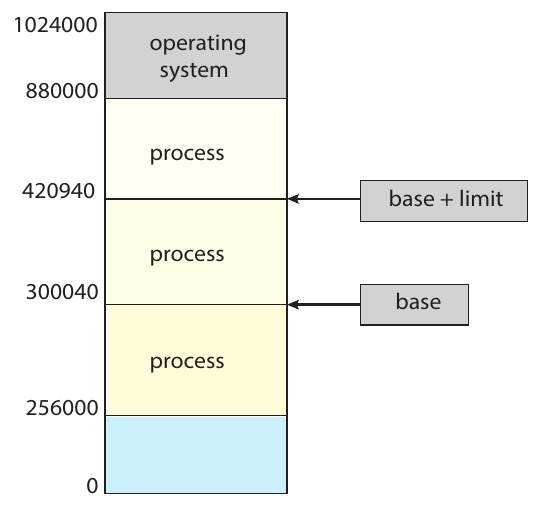
\includegraphics[width=3cm]{baseLimit.png}
	\endgroup

	\textbf{virtual address}-address after binding stage (logical mapped to physical\\
	
	\textbf{memory management unit}-maps virtual to physical addresses\\
	\begingroup
		\centering
		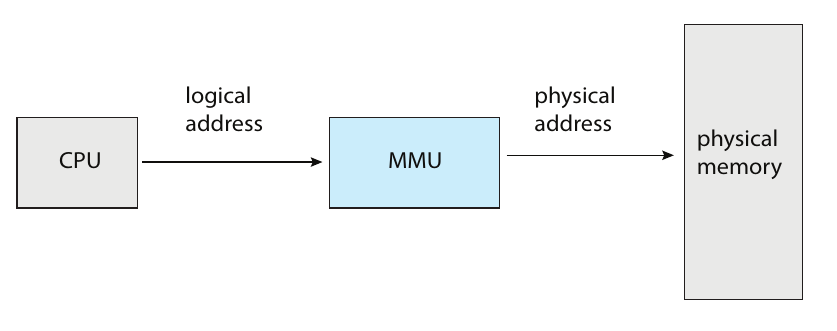
\includegraphics[width=6cm]{mmu.png}
	\endgroup
	
	\textbf{relocation register}-value is added to every addresss generated by program at the
	time that the address is sent to memory (ie if base is 14000, then accessing address 0 is 
	dynamically relocated to location 14000, or accessing 346 gets moved to 14346)\\
	\begingroup
		\centering
		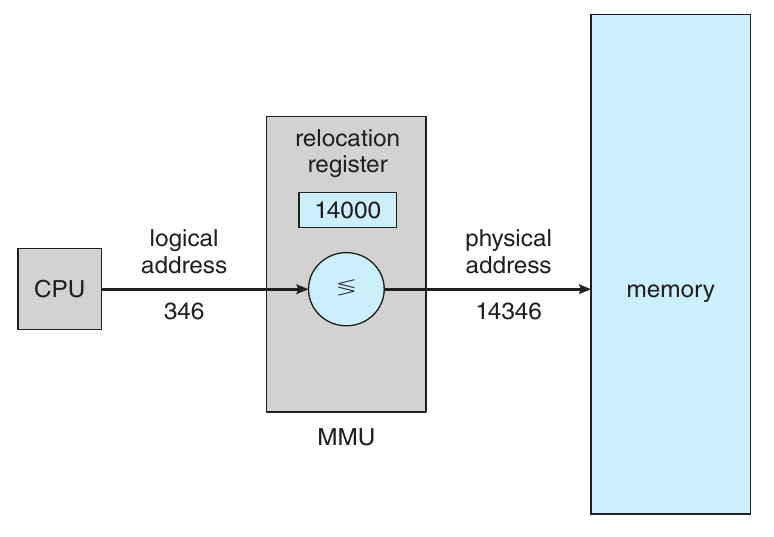
\includegraphics[width=4cm]{relocate.png}
	\endgroup
	
	\textbf{dynamic loading}-routines are not loaded into memory until they are called, useful
	in cases where routines are infrequently called (error checking)\\
	
	\subsection{Physical vs Logical memory}

	Logical Address is generated by CPU while a program is running. The logical address is virtual address as it does not exist physically, therefore, it is also known as Virtual Address. This address is used as a reference to access the physical memory location by CPU. The term Logical Address Space is used for the set of all logical addresses generated by a program’s perspective.
The hardware device called Memory-Management Unit is used for mapping logical address to its corresponding physical address.

Physical Address identifies a physical location of required data in a memory. The user never directly deals with the physical address but can access by its corresponding logical address. The user program generates the logical address and thinks that the program is running in this logical address but the program needs physical memory for its execution, therefore, the logical address must be mapped to the physical address by MMU before they are used. The term Physical Address Space is used for all physical addresses corresponding to the logical addresses in a Logical address space.

	\subsubsection{Differences Between Logical and Physical Address in Operating System}
	\begin{enumerate}[noitemsep]
		\item The basic difference between Logical and physical address is that Logical address is generated by CPU in perspective of a program whereas the physical address is a location that exists in the memory unit.
		\item Logical Address Space is the set of all logical addresses generated by CPU for a program whereas the set of all physical address mapped to corresponding logical addresses is called Physical Address Space.
		\item The logical address does not exist physically in the memory whereas physical address is a location in the memory that can be accessed physically.
		\item Identical logical addresses are generated by Compile-time and Load time address binding methods whereas they differs from each other in run-time address binding method. Please refer this for details.
		\item The logical address is generated by the CPU while the program is running whereas the physical address is computed by the Memory Management Unit (MMU).
	\end{enumerate}

	\subsection{Swapping}
	Physical memory space is finite, and physical memory is allocated to meet the needs of a 
	process. What happens if total physical memory space requested by processes exceeds physical
	memory?

	A process can be swapped out of memory temporarily, moved to a disk large enough to hold
	copies of all memory images for all users. Later brought back for execution.

	Swapping is used along with process scheduling.

	\textbf{Roll out, roll in} is a swapping
	variant used with priority scheduling. Lower priority processes get swapped out so higher
	ones can execute.

	Transfer time for swapping is directly proportional to the amount of memory swapped. 

	System maintains a ready queue of processes that have memory images on disk.
	
	\subsection{Allocation}
	
		\subsubsection{Contiguous versus non-contiguous}
		Memory is divided into two paritions, OS and user. OS memory can be either the high chunk
		or the low chunk (Linux and Windows go high).\\
		\textbf{contiguous memory allocation}-each process has a chunk of memory that is 
		contiguous to the section containing the next process\\
		
		\textbf{variable-parition}-allocating memory by assigning processes to variably sized 
		partitions in memory, where each parition may contain a single process\\
		\begingroup
			\centering
			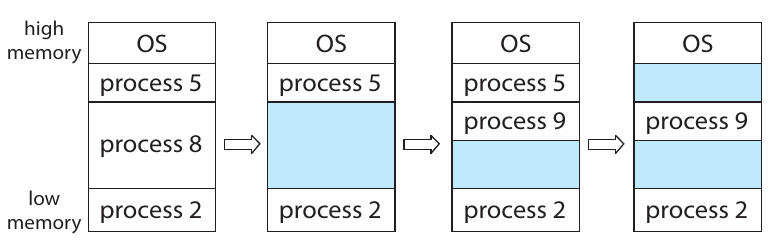
\includegraphics[width=6cm]{varPart.png}
		\endgroup
		
		When a process enters the system, OS checks to see if it has a memory block large enough
		for process. If it does not, it can either:
		\begin{itemize}[noitemsep]
			\item Send and error and reject the process
			\item Place process into a queue to wait for a proper sized chunk
		\end{itemize}

		As memory is released, OS checks if it can allocate that memory to a waiting process.
		If a hole is too large, it gets split into two parts (holes are merged if adjacent).
		As process enter and leave memory, this can result in non-contiguous holes of various sizes
		in memory.

		\textbf{dynamic storage allocation problem}-how to satisfy a request of size n from a list
		of free holes, many solutions exist:
		
		\begin{itemize}[noitemsep]
			\item \textbf{first-fit}-iterate through holes and allocate first hole >= size n
			\item \textbf{best-fit}-iterate and allocate first hole = size n
			\item \textbf{worst-fit}-iterate and allocate largest hole of at least size n
		\end{itemize}

		\textbf{First-fit} and \textbf{best-fit} are \textbf{better} than worst fit in terms of 
		speed and storage use
		
		\subsubsection{Algorithms}
		\textbf{first-fit}-Even with optization, given N blocks, another 0.5 N blocks will
		lost to fragmentation(third of memory becomes unusable \textbf{50-percent rule})
		
	
	\subsection{Fragmentation}
		\subsubsection{External}
		Both \textbf{first-fit} and \textbf{best-fit} suffer from \textbf{external fragmentation}.

		\textbf{external fragmentation}-occurs when there is enough free memory space to satisfy
		a request, but available memory is not contiguous, it is broken into smaller pieces

		\textbf{compaction}-shuffling memory contents so all the free blocks of memory are placed
		as a large block. This is not possible if relocation is static and done at
		assembly or load time. Compaction can only be done if relocation is dynamic and done at
		execution time.

		Relocating dynamically only requires moving the program data and then adjusting its base
		register to reflect the new base address.

		When compaction is possible, cost must be determined. A simple algorithm will move all 
		processes to one end in memory, and all holes to the other, forming one large hole of 
		memory. This can be expensive to run.
		
		\subsubsection{Internal}
		\textbf{internal fragmentation}-when breaking memory into fixed sized blocks, you allocate
		a block to a process that is bigger than its memory demand. Difference in memory is 
		\textbf{internal} to partition, but not being used.

\section{Paging}
	\textbf{paging}-memory management scheme that permits a processs's physical address space
	to be non-contiguous

	Paging avoids external fragmentation and need for compaction, the two main problems with
	contiguous memory allocation. Paging works via cooperation between the OS and hardware.

	\textbf{frame}-fixed size block of physical memory
	
	\textbf{page}-fixed size block of logical memory

	Every address generated by the CPU is broken into a \textbf{page number} and a 
	\textbf{page offset}
	
	\begingroup
		\centering
		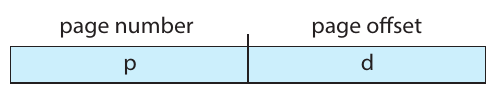
\includegraphics[width=4cm]{page.png}
	\endgroup
	
	\begingroup
		\centering
		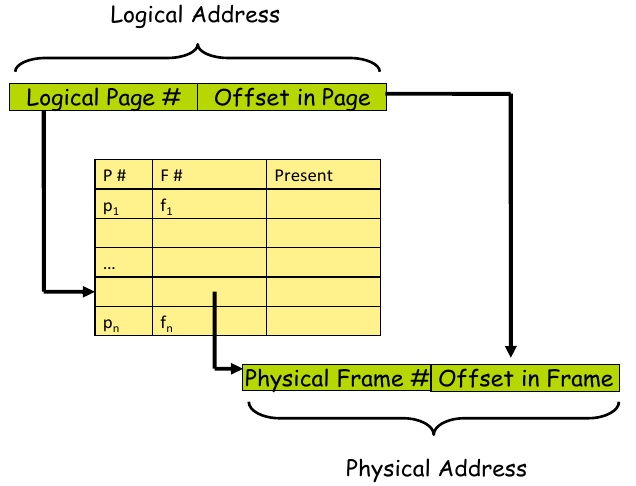
\includegraphics[width=6cm]{pageTable.png}
	\endgroup

	\textbf{page table}-contains the base address of each frame in physical memory, and 
	the offset is the location in each frame being referenced
	
	\subsection{Virtual-physical translation}
	
	\begin{itemize}[noitemsep]
	   \item Programs are provided with a logical address space
	   \item Role of the OS is to fetch data from either physical memory or disk (done by paging)
	   \item Divide the logical addrress space into units called (logical) pages, each of which 
		   is of fixed size (usually 4k or 8k)
	   \item Divide physical address space into (physical) frames
	\end{itemize}
	
	\begingroup
		\centering
		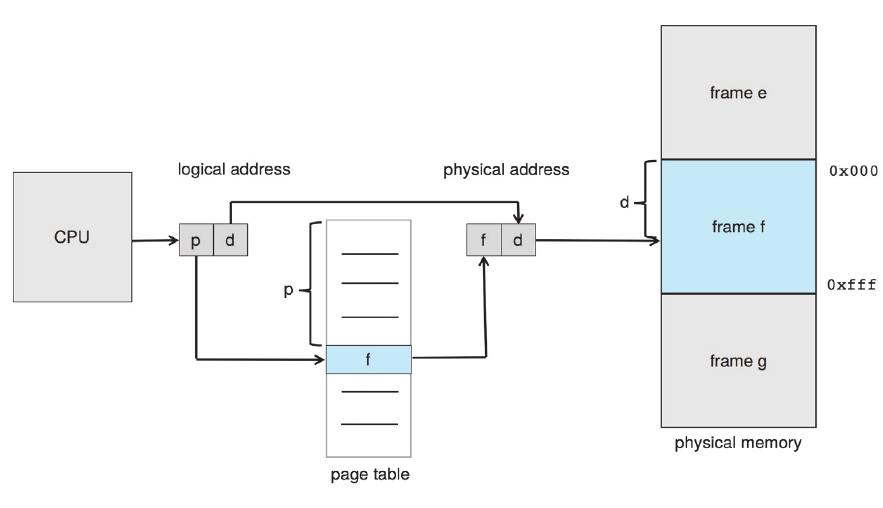
\includegraphics[width=7cm]{pageHW.png}
	\endgroup

	\begin{enumerate}[noitemsep]
		\item Extract page number {\it p} and use as index into the page table
		\item Extract the corresponding frame number {\it f} from the page table
		\item Replace the page number {\it p} in the logical address with the frame number {\it f}
	\end{enumerate}

	The offset {\it d} does not change or become replaced, the frame number {\it f} and the offset
	now comprise the physical address.

	Page size is defined by hardware (usually a power of 2 between 512 bytes and 16 Mbytes). 
	Using a power of 2 allows easy translating from logical address to page number and page 
	offset easy.

	If logical address space is $2^m$ and page size is $2^n$ bytes, then the high order
	$m-n$ bits of a logical address desginate the page number, and the $n$ lower order bits
	of a logical address designate the page offset. So the logical address is as follows:
	
	\begingroup
		\centering
		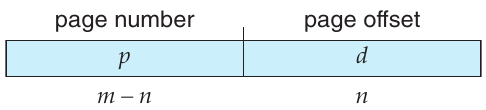
\includegraphics[width=4cm]{pageTrans.png}
	\endgroup
	
	\subsubsection{Page Map Example}

	\begin{itemize}[noitemsep]
		\item Given logical address $n=2$ and $m=4$.
		\item Using a page size of 4 bytes and a physical memory of 32 bytes (8 pages).
		\item Logical address is page 0, offset 0
		\item Page 0 is in frame 5
		\item Thus logical address 0 maps to physical address 20 ($5x4+0$)
		\item Thus logical address 3 maps to physical address 23 ($5x4+3$)
		\item Logical address 4 is page 1, offset 0 and page 1 is mapped to fram 6
		\item Thus logical address 3 maps to physical address 24 ($6x4+0$)
	\end{itemize}

	\subsection{Paging and Fragmentation}

	Paging has no external fragmentation, but can have internal (allocating an amount of pages
	equal to more memory than a program needs).
	
	\subsubsection{Internal Fragmentation Calculation}
	\begin{itemize}[noitemsep]
		\item Page size = 2048 bytes
		\item Process size = 72766 bytes
		\item 35 pages + 1086 bytes
		\item Internal Frag of 2048 - 1086 = 962 bytes
		\item Worst case frag = 1 frame - 1 byte
		\item Average case frag = 1/2 frame size
	\end{itemize}
	Are small frames desirable? Not really, becuase smaller frames need more page tables, and
	those take memory to track. Page sizes are growing over time.

	\textbf{frame table}-system wide table detailing frames allocated to physical memory, and if
	it is free

	\subsection{Implementation of Page Table}
	Page table is kept in main memory
	\subsection{Translation Look Aside Buffer}

	The idea used here is, place the page table entries in registers, for each request generated from CPU (virtual address), it will be matched to the appropriate page number of the page table, which will now tell where in the main memory that corresponding page resides. Everything seems right here, but the problem is register size is small (in practical, it can accommodate maximum of 0.5k to 1k page table entries) and process size may be big hence the required page table will also be big (lets say this page table contains 1M entries), so registers may not hold all the PTE’s of Page table. So this is not a practical approach.

To overcome this size issue, the entire page table was kept in main memory. but the problem here is two main memory references are required:

    To find the frame number
    To go to the address specified by frame number

To overcome this problem a high-speed cache is set up for page table entries called a Translation Lookaside Buffer (TLB). Translation Lookaside Buffer (TLB) is nothing but a special cache used to keep track of recently used transactions. TLB contains page table entries that have been most recently used. Given a virtual address, the processor examines the TLB if a page table entry is present (TLB hit), the frame number is retrieved and the real address is formed. If a page table entry is not found in the TLB (TLB miss), the page number is used to index the process page table. TLB first checks if the page is already in main memory, if not in main memory a page fault is issued then the TLB is updated to include the new page entry.


\textbf{Steps in TLB hit:}
\begin{enumerate}[noitemsep]
	\item CPU generates virtual address.
    \item It is checked in TLB (present).
    \item Corresponding frame number is retrieved, which now tells where in the main memory page lies.
\end{enumerate}

\textbf{Steps in Page miss:}
\begin{enumerate}[noitemsep]
	\item CPU generates virtual address.
    \item It is checked in TLB (not present).
    \item Now the page number is matched to page table residing in main memory (assuming page table contains all PTE).
    \item Corresponding frame number is retrieved, which now tells where in the main memory page lies.
    \item The TLB is updated with new PTE (if space is not there, one of the replacement technique comes into picture i.e either FIFO, LRU or MFU etc).
\end{enumerate}

\textbf{Effective memory access time(EMAT)} : TLB is used to reduce effective memory access time as it is a high speed associative cache.
\textbf{EMAT = h*(c+m) + (1-h)*(c+2m)}
where, h = hit ratio of TLB
m = Memory access time
c = TLB access time 





\section{Virutal Memory}
	\subsection{What is virtual memory}
	\textbf{virtual memory}-is the seperation of logical memory from physical memory. 
	Virtual memory takes \textbf{program addresses} and \textbf{maps} them to 
	\textbf{physical addresses}
	
	\subsubsection{Benefits}
	\begin{itemize}[noitemsep]
		\item Programs with memory needs larger than physical memory
		\item Allows sharing of address space by several processes
		\item More efficient process creation
		\item Less I/O needed to swap/load processses
		\item Libraries can be shared by processes through shared memory pages
		\item Processes can share memory regions
		\item Page can be shared during process creation with the fork() system call
	\end{itemize}

	\textbf{virutal address space}-refers to the logical/virtual view of how a process is stored
	in memory
	
	\begingroup
		\centering
		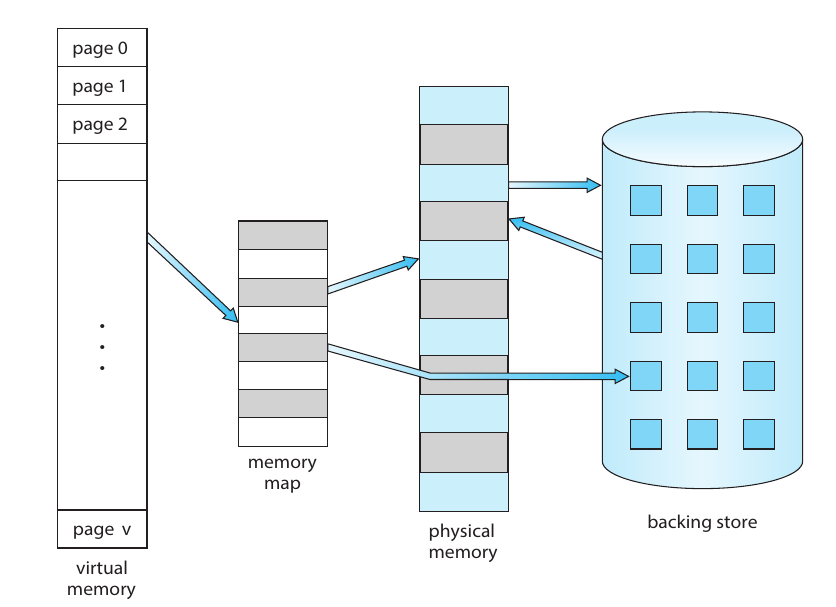
\includegraphics[width=7cm]{virtualMem.png}
	\endgroup

	\textbf{demand paging}-loading pages only when demanded by program execution
	\begin{itemize}[noitemsep]
		\item Less I/O needed
		\item Less memory
		\item Faster reponse
		\item More users
	\end{itemize}

	\textbf{effective access time}-allowing for $0<=p<=1$ to be the probability of a page fault
	($p=0$ never faults, $p=1$ always faults), and memory access time $ma$ to be $10$ nanoseconds;
	\begin{itemize}[noitemsep]
		\item EAT $= (1-p)*ma+p*$page fault time
	\end{itemize}

	\subsection{Page fault handling}

	\textbf{page fault}-when a process tries to access a page that was not brought into memory
	\begin{enumerate}[noitemsep]
		\item Service page fault interrupt
		\item Read in the page
		\item Restart the process
	\end{enumerate}
	
	\begingroup
		\centering
		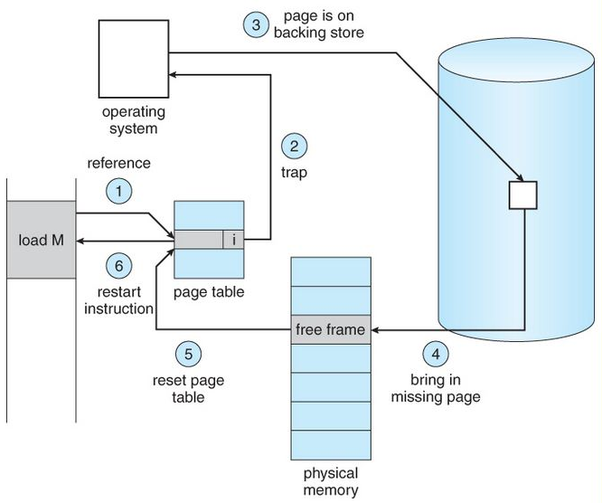
\includegraphics[width=7cm]{pageFault.png}
	\endgroup
	
	\textbf{pure demand paging}-processes are started with no pages in memory, only bringing them
	into memory after every page fault

	\textbf{free-frame list}-pool of free frames for filling page fault request

	\textbf{zero fill on demand}-frames are zeroed out before allocation, erasing contents
	(security issue)

	\begin{enumerate}[noitemsep]
		\item Trap to OS
		\item Save registers and process state
		\item Determine if interrupt was a page fault
		\item Check if page reference was legal, and determine location of page in the
			secondary storage
		\item Issue a read from the storage to a free frame
			\begin{itemize}[noitemsep]
				\item Wait in queue for request to be serviced
				\item Wait for the device seek/latency time
				\item Begin transfer of page to free frame
			\end{itemize}
		\item While waiting, allocate CPU core to another process
		\item Receive an interrupt from the storage I/O subsystem (I/O completed)
		\item Save the registers and process state for process if step 6
		\item Correct the page table and other tables to show that the desired page is now in
			memory
		\item Wait for the CPU to be allocated to this process
		\item Restore the register, process state, and new page table, then resume interrupted
			instruction
	\end{enumerate}

		\subsubsection{Performance estimations}
		\textbf{Effective access time} is directly proportional to the page fault rate
		\subsubsection{Demand Paging Example}
		\begin{itemize}[noitemsep]
			\item Memory access time = $200$ nanoseconds
			\item Average page fault service time = $8$ ms
			\item EAT $=(1-p) * 200 + p * 8000000$\\
				$=200 + p x 7999800$
			\item If one access out of every $1000$ causes a page fault, then EAT = $8.2us$
			\item Slowdown factor of 40
			\item For performance degredation below $<10$ percent \\
				$220>200 + 7999800 * p$\\
				$20 > 7999800 * p$
				$p < .0000025$ \\
				$<$ one page fault for every $400000$ memory accesses
		\end{itemize}
		
		\subsubsection{Demand Paging Opimizations}
		\begin{itemize}[noitemsep]
			\item Swap space I/O faster than file system I/O even on same device\\
				Swap sapce is allocated in larger chunks, less management needed
			\item Copy entire process image to swap space at process load time\\
				Then page in and out of swap space
			\item Demand page in from program binary on disk, but discard rather than 
				paging out when freeing frame
		\end{itemize}
		
		\subsubsection{Memory Initialization}

	\subsection{Page Replacement}
	\begin{itemize}[noitemsep]
		\item Prevent over allocation of memory by modifying page fault routine to include
			page replacement
		\item Use \textbf{modify (dirty)} bit to reduce overhead of page transfer - only 
			modified pages are written to disk
		\item Page replacement compeletes seperation between logical and physical memory - large
			virtual memory can be provided on a smaller physical memory
	\end{itemize}
		\subsubsection{Basic Page Replacement}
		\begingroup
			\centering
			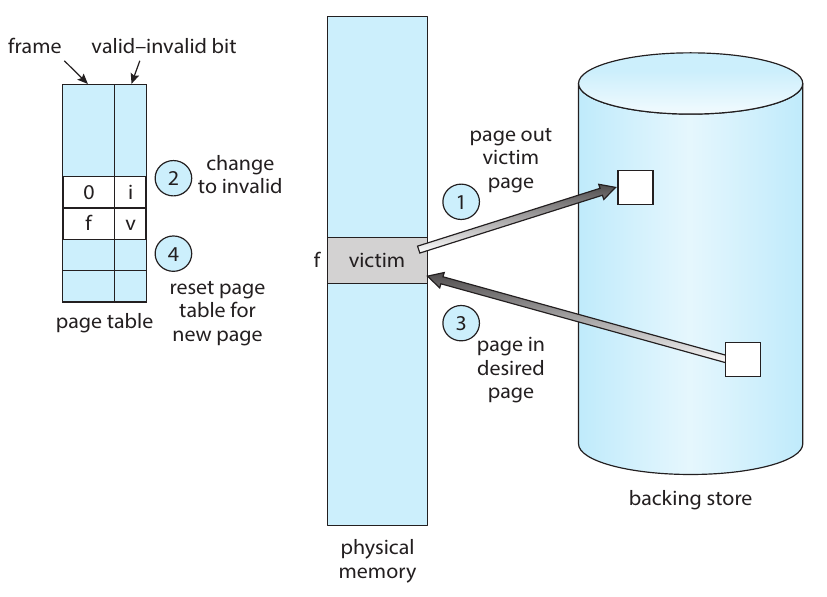
\includegraphics[width=7cm]{pageReplace.png}
		\endgroup
		\begin{enumerate}[noitemsep]
			\item Find location of desired page on secondary storage
			\item Find a free frame
				\begin{itemize}[noitemsep]
					\item If there is a free frame, use it
					\item If there is no free frame, use page-replacement algorithm to select
						a \textbf{victim frame}
					\item Write the victim frame to secondary storage (if needed); change the page
						and frame tables accordingly
				\end{itemize}
			\item Read the desired page into the newly freed frame; change the page and frame
				tables
			\item Continue the process from where the page fault occured
		\end{enumerate}
		If no frames are free, \textbf{two} page transfers (one for page out and one for page in) 
		are required - increasing \textbf{EAT}.

		Overhead can be reduced by using a modify bit (or dirty bit). Each frame/page gets a bit
		asscociated with it in the hardware.

		\subsubsection{Page Replacement Algorithms}
		\begin{itemize}[noitemsep]
			\item Frame-allocation algorithm determines\\
				How many frames given to each process
				Which frames to replace
			\item Page-Replacement Algorithm\\
				Want lowest page-fault rate on both first access and re-access
			\item Evaluate algorithm by running on string of memory references, and computing
				number of page faults\\
				String is page numbers, not full addresses\\
				Repeated access to same page does not cause a page fault\\
				Results depend on number of frames available
			\item In all these examples, reference string is\\
				\textbf{7,0,1,2,0,3,0,4,2,3,0,3,0,3,2,1,2,0,1,7,0,1}
		\end{itemize}

		\subsubsection{FIFO}
		\begin{itemize}[noitemsep]
			\item 3 Frames (3 pages in memory at once per process)
			\begingroup
				\centering
				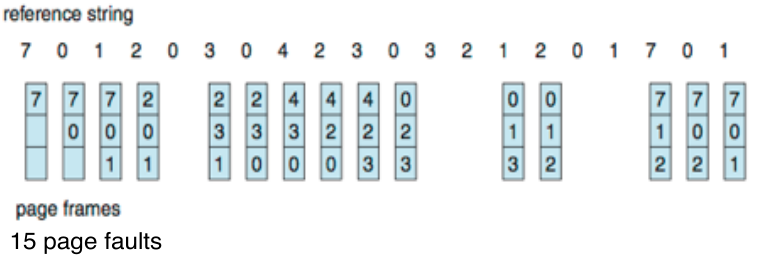
\includegraphics[width=6cm]{fifo.png}
			\endgroup
			\item Can vary by reference string: consider \textbf{1,2,3,4,1,2,5,1,2,3,4,5}\\
				Adding more frames can cause more page faults! (Belady's anomaly)
			\item How to track pages? Use a FIFO queue
		\end{itemize}
		\subsubsection{Optimal Algorithm}
		\begin{itemize}[noitemsep]
			\item Replace page that will not be used for longest period of time\\
				9 is optimal for example
			\item How do you know?
			\item Used for measuring how well algorithm performs
			\begingroup
				\centering
				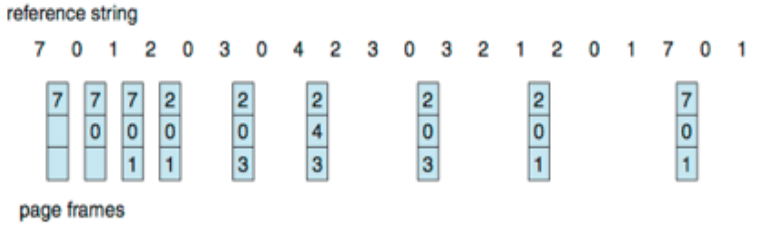
\includegraphics[width=6cm]{optimal.png}
			\endgroup
		\end{itemize}
		\subsubsection{Least Recently Used}
		\begin{itemize}[noitemsep]
			\item Use past knowledge
			\item Replace page that has not been used in the most amount of time
			\item Associate time of last use with each page
			\begingroup
				\centering
				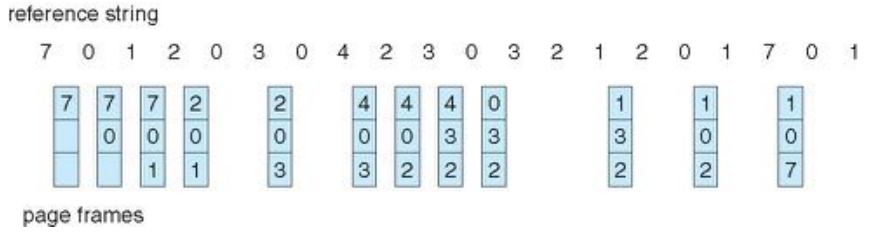
\includegraphics[width=6cm]{lru.png}
			\endgroup
			\item 12 faults - better than FIFO but worse than OPT
			\item Generally good, frequently used
			\item How to implement?
			\item Counter implementation\\
				Every page has a counter, every time a page is referenced through this entry, copy
				the clock into the counter\\
				When a page needs to be changed, check counters to find smallest value 
				(search though table needed)\\
			\item Stack implementation\\
				Keep stack of pages in double link form\\
				Page referenced, move to top (6 pointers must be changed)\\
				Each update more expensive\\
				No search to replace\\
			\item LRU and OPT are cases of stack algorithms that don't have 
				\textbf{Belady's Anomaly}
			\item LRU need special hardware and still slow
			\item Second chance algorithm\\
				Generally FIFO, hardware provided reference bit\\
				Clock replacement\\
				If page to be replaced has \textbf{ref bit = 0} then replace\\
				If \textbf{ref bit = 1} then set bit 0, leave page in memory

		\end{itemize}
		\subsubsection{Enhanced Second Chance}
		\begin{itemize}[noitemsep]
			\item Improve by using reference bit and modify bit in concert
			\item Take ordered pair
				\begin{enumerate}[noitemsep]
					\item (0,0) not recently used not modified - best page to replace
					\item (0,1) not recently used but modified - not as good, must write out
						before replacement
					\item (1,0) recently used but clean, probably will be used again soon
					\item (1,1) recently used and modified - probably will be used again soon
						and need to write out before replacement
				\end{enumerate}
    		\item When page replacement called for, use the clock scheme but use the four classes
				replace the page in lowest non-empty class\\
				Might need to search circular queue several times
		\end{itemize}
		\subsubsection{Counting}
		\subsubsection{Page Buffering}
		
		\subsubsection{Belady's anomaly}
		Bélády’s anomaly is the name given to the phenomenon where increasing the number of page 
		frames results in an increase in the number of page faults for a given memory access 
		pattern.\\
		This phenomenon is commonly experienced in following page replacement algorithms:\\
		\begin{enumerate}[noitemsep]
			\item First in first out (FIFO)
			\item Second chance algorithm
    		\item Random page replacement algorithm
		\end{enumerate}

		\textbf{Reason of Belady’s Anomaly} –
The other two commonly used page replacement algorithms are Optimal and LRU, but Belady’s Anamoly can never occur in these algorithms for any reference string as they belong to a class of stack based page replacement algorithms.

A \textbf{stack based algorithm} is one for which it can be shown that the set of pages in memory for N frames is always a subset of the set of pages that would be in memory with N + 1 frames. For LRU replacement, the set of pages in memory would be the n most recently referenced pages. If the number of frames increases then these n pages will still be the most recently referenced and so, will still be in the memory. While in FIFO, if a page named b came into physical memory before a page – a then priority of replacement of b is greater than that of a, but this is not independent of the number of page frames and hence, FIFO does not follow a stack page replacement policy and therefore suffers Belady’s Anomaly.

			\begingroup
				\centering
				\includegraphics[width=6cm]{belady.png}
			\endgroup

			\textbf{Why Stack based algorithms do not suffer Anomaly –}\\
All the stack based algorithms never suffer Belady Anomaly because these type of algorithms assigns a priority to a page (for replacement) that is independent of the number of page frames. Examples of such policies are Optimal, LRU and LFU. Additionally these algorithms also have a good property for simulation, i.e. the miss (or hit) ratio can be computed for any number of page frames with a single pass through the reference string.

In LRU algorithm every time a page is referenced it is moved at the top of the stack, so, the top n pages of the stack are the n most recently used pages.Even if the number of frames are incremented to n+1, top of the stack will have n+1 most recently used pages.
	
	\subsection{Aspects of virtual memory}
		\subsubsection{When to update: copy-on-write}
		\begin{itemize}[noitemsep]
			\item \textbf{copy-on-write}-allows both parent and child processes to intially 
				share the same pages in memory
			\item COW allows more efficient process creation as only modified pages are copied
			\item In general, free pages are allocated from a pool of 
				\textbf{zero-fill-on-demand} pages
			\item vfork() variation of fork() system call has parent suspend and child using COW
				address space of parent
		\end{itemize}
		\subsubsection{Sharing: shared pages between processors}
		
		\subsubsection{Use with I/O:memory mapped files}
	\subsection{Thrashing}
		\begin{itemize}[noitemsep]
			\item IF a process does not have enoug pages, page fault rate is very high\\
			\item Page fault to get page\\
			\item Replace existing frame\\
			\item But quickly need replaced frame back\\
			\item Leading to: low CPU utilization, OS thinking it needs to increase 
				multiprogramming, another process added to system
			\item Thrashing = a process is busy swapping pages in and out
		\end{itemize}
	\subsection{Working sets}

\section{Processes and Threads}

\begingroup
	\centering
	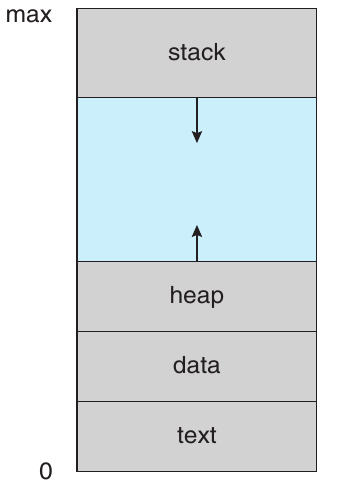
\includegraphics[width=2cm]{proc.png}
	\captionof{figure}{Process}\label{fig:c}
\endgroup

\textbf{What do the terms multiprogramming, multiprocessing, and multithreading mean? 
Is it possible to do multiprogramming if the computer system only has one processor?}

\textbf{multiprogramming}-a computer running more than one processes at a time

\textbf{multiprocessing}-a computer using more than one CPU at a time

\textbf{multithreading}-having multiple threads of execution for one process

\textbf{What is a process control block and what is its purpose?}

The process control block contains pieces of information associated with a specific process.

\textbf{Process State}-state can be new, ready, running, waiting, halted, etc

\textbf{Program Counter}-counter includes the address of the next instruction to be executed

\textbf{CPU registers}-vary in number and type, such as accumulators, indexes, stack pointers
general registers

\textbf{Schedule info}-process priority, pointers to schedule queue, and other parameters

\textbf{memory-management information}-information on base and limit registers, page tables,
or the segment tables

\textbf{accounting information}-amount of CPU and real time used, time limits, account numbers,
jobs, or process numbers

\textbf{I/O status information}-list of I/O devices allocated to the process, open files, etc

\textbf{What is the process address space? What is in it and where are things located?
Draw a picture to show this.} 

\textbf{What is the difference between 1:1 M:1 threading? Why might we prefer a 1:1 threading 
model?}

The one to one model maps each user thread to a kernel thread. Provides more concurrency than M:1,
by allowing another thead to run when a thread makes a blocking system call. It also allows 
multiple threads to run in parallel on multiprocessors. The drawback to this model is that creating
a user level thread requires creating a corresponding kernel thread, and a large number of kernel 
threads can burden the performace of a system. (Linux and Windows use 1:1)

Many to one maps many user level threads to one kernel level thread. Thread management is done by
the thread library in the user space, so it is effiecient. However, the entire process whill block
if a thread makes a blocking system call. Also because only one thread can access the kernel at a
time, multiple theads are unabble to run in parallel on a multicore system.

\textbf{Single thread vs multithreaded}

Single threaded processes have their own code, data, files, registers, PC, and stack.
The threads in a multithreaded process share code, data, and files, but have their own registers,
stack, and PC.

\textbf{What is a process? What is a thread? How do they differ?} 
A process is a program in execution. A thread is a path of execution in a program.

1) Processes have their own memory space, threads have a shared memory space. 

2) All the threads running within a process share the same address space, file descriptors, stack 
and other process related attributes. 

3)It is termed as a ‘lightweight process’, since it is similar to a real process but executes 
within the context of a process and shares the same resources allotted to the process by the 
kernel.

\textbf{OSC 4.4: What are two differences between user-level threads and kernel-level treads? Under what circumstances is one type better than the other?}

User-level threads exist entirely at the user-level.  That is, all of the common thread operations
(e.g., creation, deletion, synchronization) are implemented in user code, typically a user library.  The oper-
ating system is not involved at all, and, in fact, is completely oblivious to the existence of user-level threads.
The benefit of user-level threads is a closer coupling of thread interaction, as mainly evidenced by more
rapid, finer-grained thread switching.
Kernel-level threads,  in contrast,  are implemented in the OS kernel.   System calls are necessary for
thread creation, deletion, and so on.  Once created, kernel-level threads have similar interaction capabili-
ties as user-level threads.  A significant difference exists, however, in how the threads execute.  User-level
threads share a single process.  When the process blocks, none of the threads created as part of the process
can execute. Threads supported by the kernel share the CPU. The OS has maintained enough state for each
thread in a set of threads such that if one thread blocks, the other threads can continue to execute. Although
the overhead of thread switching is greater with kernel-level threads, a greater degree of ”real” concurrency
is allowed.

User-level threads are often used to allow a program to perform logically concurrent parts of its com-
putation without resorting to the creation of OS processes or kernel threads.  When real concurrency is not
required, user-level threads gives a low overhead way to switch between different threads of execution.  It
is also a way to achieve thread-based programming when the OS does not support threads, and user-level
thread libraries can be ported to other architectures with only a rewrite of the thread switching code.
Kernel-level threads are “better” when one expects the individual threads to have OS involvement since
the blocking of one thread (for example, due to a file I/O system call) does not automatically prevent the
other threads from proceedings, as is the case with user-level threads. Even though the overhead of kernel-
level thread switching is greater,  the improved performance that comes from concurrent execution often
more than makes up for it, especially when system call blocking is frequent.
In reality, user-level threads must be “mapped” to kernel-level threads to actually run.  In threading li-
braries, such as Pthreads, there is this mapping taking place.  It is possible in some systems to create more
user-level threads than the number of kernel-level threads assigned to a process, thereby requiring the user-
level thread scheduler to perform this mapping.

\textbf{OSC 3.5: When a process creates a new process using the
fork() operation, which of the following states
is shared between the parent process and the child process: A. Stack, B. Heap, C. Shared memory segments.
(Addition: Describe what problems might arise if the opposite were true.)}

When a parent process uses
fork()
to create a child process, the child has its own memory space.
In particular, the stack and heap part of that memory space are separate from parent (i.e., the addresses used
to reference the stack and heap in the parent and child DO NOT go to the same physical location. However,
if a shared memory segment is set up between the parent and the child, the memory segment is shared (i.e.,
the addresses used to reference the shared memory segment DO go to the same physical location). Instead, if
it were the other way round and the stack and heap were shared by each child and parent process, they could
theoretically overwrite one-another’s data in memory.  This would likely lead to unexpected and incorrect
behavior that could cause the processes to function incorrectly.

\textbf{What happens during a context switch?}

When an interrupt occurs, the system needs to save the context of the processes running on the CPU,
so that context can be restored.

This includes the value of the CPU registers, process state, and memory management info.

Generally, perform a save state of CPU (in kernel or user) and then save restore to resume.

Switching the CPU between processes is called a context switch. Context switching has a lot of 
overhead, because the system does no work while switching.

\textbf{What is a process control block and what is its purpose?}

It serves as a repository for all data needed to start or restart a proecess.

A process control block represents processes by storing relevant information, such as:

1) Process state: State may be new, ready, running, waiting, halted, etc

2) Program counter: Indicates address of the next instruction.

3) CPU Registers

4) CPU scheduling info: Process priority, pointers to schedule queues, other parameters.

5) Memory management info: Values for base and limit registers, page/segment tables, memory system

6) Accounting info: CPU/Real time used, time limits, account numbers, process numbers

7) I/O status: I/O devices allocated to process, list of open files, etc

\begingroup
	\centering
	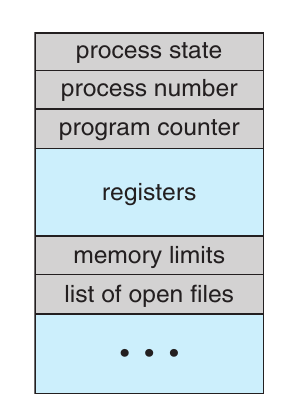
\includegraphics[width=2cm]{PCB.png}
	\captionof{figure}{Philo}\label{fig:b}
\endgroup

\textbf{What do the fork(), exec(), and clone() system calls do?}

\textbf{fork()}: Used to make new processes, that are the child of the caller. 
After fork call, BOTH processes will execute the next statement. Takes no arguments and 
returns a process ID.

\textbf{exec()}: Used to replace the process's memory space with a new program.

\textbf{clone()}: Makes threads.

\section{Deadlocks}
\subsection{Concepts}

\textbf{What are the conditions for a deadlock to occur?}

When a waiting thread never changes state because it is waiting for resources that are requested by other 
waiting threads.

In normal mode of operation, a thread may utilize a resource in only the following sequence:

1) Request: The thread requests the resource. If it cannot be granted immediately (such as if a mutex lock
is currently held by another thread), then the requesting thread must wait until it can aquire the resource.

2) Use: The thread operates on the resource (such as a mutex lock, so the thread can access its 
critical 
section).

3) Release: The thread releases the resource.

Conditions for deadlock:

\textbf{1) Mutual exclusion}: At least one resource is hold in a non-sharable mode, only on thread 
at a time can uset the resource. If another thread requests that resource, the requesting thread 
must be delayed until the resource has been released.

\textbf{2) Hold and wait}: A thread must be holding at least one resource and waiting to aquire additional resources that are being held by other threads.

\textbf{3) No preemption}: Resources cannot be preempted, that is a resource can be released only 
by the thread holding it, after that thread has completed its task.

\textbf{4) Circular wait}: A set of waiting threads must exist such that 

\section{Synchronization}

\subsection{Concepts}

\textbf{race condition}-a situation when several processses access and manipulate the same data
concurrently

\textbf{entry section}-portion of code where a process requests entry into its critical section

\textbf{exit section}-portion of code where a process exits its critical section

\textbf{What does mutual exclusion mean?}

If a process is entering its critical section, then no other process can be executing their 
critical section.

\textbf{What is a critical section? List the requirements for a solution to the critical section 
problem.}

A critical section is a segment of code in which a process may be accessing/updating data that is
shared by at least one other process. The critical section problem is to define a protocol that 
processes can use to sync activity and share data.

The requirements are:

\textbf{1) Mutual exclusion}: If a process is entering its critical section, then no other 
process can be executing their critical section.

\textbf{2) Progress}: If a process is executing in its critical section and some processes wish 
to enter their critical section, then only processes that are not executing in their remainder 
sections can participate in deciding which will enter its critical section next, and selection 
cannot be postponed indefinitely.

\textbf{3) Bounded Waiting}: There exists a bound, or limit on the number of times that other 
processes can enter their critical sections after a process has made a request to enter its 
critical section and before that request is granted.


\textbf{What is the difference between deadlock prevention and deadlock avoidance?}

Deadlock prevention techniques do not allow (prevent) deadlocks from occurring by ensuring that at least oneof the necessary conditions cannot hold.

Deadlock avoidance techniques use information about the state of resource assignments and resource requeststo control resource allocation, thereby avoiding possible future deadlocks

\textbf{preemptive kernel}-allows a process to be preempted while it is running in kernel mode

\textbf{nonpreemptive kernel}-does not allow a process a process running in kernel mode to be
preempted

\textbf{What is the difference between busy waiting and blocking?}

Busy waiting is a practice that allows a thread or process to use CPU time continuously while 
waiting for something. An I/O loop in which an I/O thread continuously reads status info while 
waiting for I/O to compile. Busy waiting wastes CPU cycles.

Blocking is where a process gives up the CPU and is wakened later when a condition is found to be 
true. Blocking does not use the CPU, where as busy waiting keeps it in a tight loop.

\textbf{mutex lock}-Mutual exclusion lock to protect critical sections and thus prevent race 
conditions. A process must aquire a lock before entering a critical section, and its releases the
lock when when it exits its critical section.

\begin{verbatim}
while (true) {
	acquire() lock
        critical section
	release() lock
        remainder section
}

acquire() {
    while (!available)
        ; /* busy wait */
    available = false;
}

release() {
    available = true;
}
\end{verbatim}


\textbf{Semaphore}-an integer variable, that apart from intialization, is accessed only through
two standard atomic instructions: \textbf{wait()} and \textbf{signal()}

\begin{verbatim}
wait(S) {
    while (S <= 0)
        ; // busy wait
    S--;
}

signal(S){
    S++;
{
\end{verbatim}

\textbf{counting semaphore}-can range over any unrestricted domain

\textbf{binary semaphore}-can range only from 0 to 1, behaves similarly mutex locks

\subsection{Peterson's Solution}

\begin{verbatim}
while (true) {
    flag[i] = true;
    turn = j;
    while (flag[j] && turn == j)
        ;
        /* critical section */

    flag[i] = false;

    /*remainder section */
}
\end{verbatim}

\textbf{Mutual Exclusion}-Note that each process enters its critical section only if either 
flag[j]==false or turn==i. Also note that if both processes can be executing their critical 
section at the same time, then flag[0] == flag[1] == true. This implies that both processes could
not have successfully executed their while statements at the same time, since the value of turn
can be either 0 or 1 but not both. Hence, one of the processes—say, Pj —must have successfully 
executed the while statement, whereas Pi had to execute at least one additional statement 
(“turn == j”). However, at that time, flag[j] == true and turn == j, and this condition
will persist as long as Pj is in its critical section; as a result, mutual exclusion is
preserved.

\textbf{Progress and Bounded waiting}-A process P can only be prevented from enterting its critical section only if it
is stuck in the while loop with condition flag[j] == true and turn == j; this loop is the only one
possible. If Pj is not ready to enter its critical section, then flag[j] == false, and Pi can 
enter its critical section. If Pj has set flag[j] to true and is also executing in its while
statement, then either turn == i or turn == j. If turn == i, then Pi will enter its critical 
section. If turn == j, then Pj will enter its critical section. However, once Pj exits its 
critical section, it will reset flag[j] to false, allowing Pi to enter its critical section. If
Pj resets flag[j] to true, it must also set turn to i. Thus, since Pi does not change the value
of the variable turn while executing the while statement, Pi will enter its critical section 
\textbf{(progress)} after at most one entry by Pj \textbf{(bounded waiting)}.

\subsection{Mutex vs Semaphore}

Consider the standard producer-consumer problem. Assume, we have a buffer of 4096 byte length. A producer thread collects the data and writes it to the buffer. A consumer thread processes the collected data from the buffer. Objective is, both the threads should not run at the same time.

\textbf{Using Mutex}

A mutex provides mutual exclusion, either producer or consumer can have the key (mutex) and proceed with their work. As long as the buffer is filled by producer, the consumer needs to wait, and vice versa.

At any point of time, only one thread can work with the entire buffer. The concept can be generalized using semaphore.

\textbf{Using Semaphore}

A semaphore is a generalized mutex. In lieu of single buffer, we can split the 4 KB buffer into four 1 KB buffers (identical resources). A semaphore can be associated with these four buffers. The consumer and producer can work on different buffers at the same time.

\textbf{Misconception}

There is an ambiguity between binary semaphore and mutex. We might have come across that a mutex is binary semaphore. But they are not! The purpose of mutex and semaphore are different. May be, due to similarity in their implementation a mutex would be referred as binary semaphore.

Strictly speaking, a mutex is locking mechanism used to synchronize access to a resource. Only one task (can be a thread or process based on OS abstraction) can acquire the mutex. It means there is ownership associated with mutex, and only the owner can release the lock (mutex).

Semaphore is signaling mechanism (“I am done, you can carry on” kind of signal). For example, if you are listening songs (assume it as one task) on your mobile and at the same time your friend calls you, an interrupt is triggered upon which an interrupt service routine (ISR) signals the call processing task to wakeup.

\textbf{General Questions}

\textbf{1. Can a thread acquire more than one lock (Mutex)?}

Yes, it is possible that a thread is in need of more than one resource, hence the locks. If any lock is not available the thread will wait (block) on the lock.

\textbf{2. Can a mutex be locked more than once?}

A mutex is a lock. Only one state (locked/unlocked) is associated with it. However, a recursive mutex can be locked more than once (POSIX complaint systems), in which a count is associated with it, yet retains only one state (locked/unlocked). The programmer must unlock the mutex as many number times as it was locked.

\textbf{3. What happens if a non-recursive mutex is locked more than once.}

Deadlock. If a thread which had already locked a mutex, tries to lock the mutex again, it will enter into the waiting list of that mutex, which results in deadlock. It is because no other thread can unlock the mutex. An operating system implementer can exercise care in identifying the owner of mutex and return if it is already locked by same thread to prevent deadlocks.

\textbf{4. Are binary semaphore and mutex same?}

No. We suggest to treat them separately, as it is explained signalling vs locking mechanisms. But a binary semaphore may experience the same critical issues (e.g. priority inversion) associated with mutex. We will cover these in later article.

A programmer can prefer mutex rather than creating a semaphore with count 1.

\textbf{5. What is a mutex and critical section?}

Some operating systems use the same word critical section in the API. Usually a mutex is costly operation due to protection protocols associated with it. At last, the objective of mutex is atomic access. There are other ways to achieve atomic access like disabling interrupts which can be much faster but ruins responsiveness. The alternate API makes use of disabling interrupts.

\textbf{6. What are events?}

The semantics of mutex, semaphore, event, critical section, etc… are same. All are synchronization primitives. Based on their cost in using them they are different. We should consult the OS documentation for exact details.

\textbf{7. Can we acquire mutex/semaphore in an Interrupt Service Routine?}

An ISR will run asynchronously in the context of current running thread. It is not recommended to query (blocking call) the availability of synchronization primitives in an ISR. The ISR are meant be short, the call to mutex/semaphore may block the current running thread. However, an ISR can signal a semaphore or unlock a mutex.

\textbf{8. What we mean by “thread blocking on mutex/semaphore” when they are not available?}

Every synchronization primitive has a waiting list associated with it. When the resource is not available, the requesting thread will be moved from the running list of processor to the waiting list of the synchronization primitive. When the resource is available, the higher priority thread on the waiting list gets the resource (more precisely, it depends on the scheduling policies).

\textbf{9. Is it necessary that a thread must block always when resource is not available?}

Not necessary. If the design is sure ‘what has to be done when resource is not available‘, the thread can take up that work (a different code branch). To support application requirements the OS provides non-blocking API.

For example POSIX pthread-mutex-trylock() API. When mutex is not available the function returns immediately whereas the API pthread-mutex-lock() blocks the thread till resource is available.

\subsection{Dining Philosopher}

The Dining Philosopher Problem – The Dining Philosopher Problem states that K philosophers seated around a circular table with one chopstick between each pair of philosophers. There is one chopstick between each philosopher. A philosopher may eat if he can pickup the two chopsticks adjacent to him. One chopstick may be picked up by any one of its adjacent followers but not both.

\begingroup
	\centering
	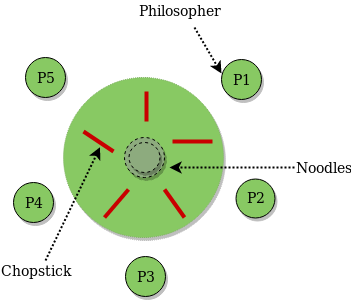
\includegraphics[width=5cm]{philo.png}
	\captionof{figure}{Philo}\label{fig:a}
\endgroup

Each philosopher is represented by the following pseudocode:

\begin{verbatim}
process P[i]
 while true do
   {  THINK;
      PICKUP(CHOPSTICK[i], CHOPSTICK[i+1 mod 5]);
      EAT;
      PUTDOWN(CHOPSTICK[i], CHOPSTICK[i+1 mod 5])
   }
\end{verbatim}

There are three states of philosopher : THINKING, HUNGRY and EATING. Here there are two semaphores : Mutex and a semaphore array for the philosophers. Mutex is used such that no two philosophers may access the pickup or putdown at the same time. The array is used to control the behavior of each philosopher. But, semaphores can result in deadlock due to programming errors.


%\begingroup
%	\centering
%	\includegraphics[width=8cm]{rbdelete11.png}
%	\captionof{figure}{Simple Case}\label{fig:a}
%\endgroup

\end{tiny}

\end{multicols}
\end{document}
